\documentclass[a4paper]{article}  

\usepackage[utf8]{inputenc}
\usepackage[ngerman]{babel}	
\usepackage[babel,german=quotes]{csquotes}
%\usepackage[none]{hyphenat}
\usepackage{listings}
\usepackage{graphicx}
\usepackage{float}
\usepackage[hidelinks]{hyperref}
\usepackage{geometry}
\usepackage{wallpaper}
% may add sorting=nty later
\usepackage[backend=bibtex]{biblatex}
\usepackage{tocloft}
\parindent0pt

\geometry{
	a4paper, 
	top=25mm,
	left=40mm,
	right=25mm,
	bottom=30mm,
	headsep=10mm,
	footskip=12mm
} 

\defbibheading{head}{\section{Quellenverzeichnis}}
\addbibresource{../Zitate/zitate.bib}

\begin{document}

	\begin{titlepage}
		\topmargin12cm
		\ULCornerWallPaper{1}{../Bilder/Header.jpeg}
		\begin{flushright}	
			{\large Masterarbeit \\}
			\begin{Large}
				\textbf{
					Ein System zur partiellen Synchronisation \\ 
					von Wissensbasen für dezentrale soziale Netzwerke \\
				} 
			\end{Large}
			\vspace{1.0cm}
			\begin{large}	
				von Jens Grundmann \\
				\today \\
				\vspace{1.0cm}
				Hochschule für Technik und Wirtschaft Berlin \\
				Fachbereich Wirtschaftswissenschaften II \\
				Studiengang Angewandte Informatik \\
				\vspace{1.0cm}
				Erstgutachter/in Prof. Vorname Name \\
				Zweitgutachter/in Vorname Name \\	
				\vspace{0.5cm}
				\begin{center}
					
\includegraphics{../Bilder/htw_logo.jpg}
				\end{center}				
			\end{large}
		\end{flushright}	
	\end{titlepage}
	
	\ClearWallPaper	
	\newpage
	
	
	%{\LARGE \textbf{Insert later}}
	%\begin{itemize}
		%\item \hyperref[sec:sharkthemes]{Themen Shark Framework}.
	%\end{itemize} 	
	
	\newpage	
	\tableofcontents
	\newpage


	\section{Einleitung}
	
	Soziale Netzwerke erfreuen sich immer mehr Beliebtheit in den letzten Jahren. 
	Sei es Facebook oder schlicht das Forum zum Online Game, dass man gerade
	spielt. Der Mensch möchte sich austauschen. Allerdings spätestens seit den
	Enthüllungen Edward Snowdens gegen Ende Mai 2013 stellt sich hier die Frage
	der Sicherheit der persönlichen Daten. Die meisten sozialen Netzwerke basieren
	auf einer Client-Server Architektur. Dies beutetet, dass alle Daten auf einem
	entfernten Server gespeichert sind. Der Nutzer hat somit keine Kontrolle bzw.
	nur die beschränkte Kontrolle, welche der Betreiber des sozialen Netzwerkes
	anbietet, wie mit seinen Daten umgegangen wird. \\
	
	Dies ist Motivation für ein Umdenken. Anstatt die Daten an zentraler Stelle
	zu speichern verbleiben sie auf den lokalen Systemen der Benutzer. Das
	Client-Server Modell wird durch ein Peer to Peer Model ersetzt. Daten
	werden nur mit den Personen ausgetauscht, für die sie bestimmt sind.
	Hier ist eine Methode benötige, welche die Daten der lokalen Systeme
	mit einander synchronisiert. \\

	Ziel dieser Arbeit ist es eine Softwarekomponente zu entwickeln, die eine 
	partiellen Synchronisation von Wissensbasen ermöglicht. Eine Wissensbasis
	ist dabei nichts anderes als ein eine Menge an Daten, die in einer
	bestimmten Stuckatur vorliegen bzw. durch eine abstrakte Darstellung
	beschreibbar sind. Mittels dieser abstrakte Darstellung soll die 
	Implementierung von Chats, Foren bis hin zu Source Code Management Systemen
	auf einer Peer to Peer Basis vereinfacht werden.
	Als Grundlage dient hierzu das Shark Framework \cite{SharkFW} von Prof.
	Dr.	Thomas Schwotzer und die darin enthalte SyncKB Klassensammlung. Diese
	ermöglicht bereits eine Synchronisation aller Daten in einer Wissensbasis.
	Diese soll nun dahingehen ausgebaut werden, dass Teile der Wissensbasis
	beschrieben werden können und nur diese beschrieben Teile synchronisiert 
	werden. \\
	
	Zuerst muss mit eine Möglichkeit gefunden werden, wie ein Teilbereich der
	Wissensbasis beschrieben werden kann. Diese müssen dann	zwischen den 
	einzelnen Peers kommunizierbar und auf den lokalen Systemen der Peers
	persistierbar sein. Die durch diese Beschreibungen extrahierten Daten
	werden synchronisiert, wobei der Peer auf diese Aktion regieren kann um
	sie beispielsweise in einer grafischen Oberfläche auszugeben. Hierbei
	ist darauf zu achten, dass die Beschreibung so abstrakt gewählt wird, dass 
	sie	auf möglichst viele Fälle, wie die erwähnte Möglichkeit der 
	Implementierung von Chats oder Foren, anwendbar ist. \\à
	Als Beweis der Funktionalität der Softwarekomponente wird schließlich
	eine Chat mit grafisch Oberfläche geschrieben, in dem einzelne Peers sich
	miteinander	unterhalten können.\\
	
	Die Arbeit wird zuerst die Grundlagen, wie das Shark Framework \cite{SharkFW},
	auf denen die Implementierung beruht, erläutern. Danach wird das Konzept
	der Softwarekomponente erstellt. Es werden verschieden Möglichkeit
	diskutiert, um die im letzten Absatz beschriebenen Anforderungen umzusetzen.
	Im Anschluss wird die eigentliche Implementierung vorgestellt und auf
	diese eingegangen. Nachfolgend werden die Tests und Methoden nur
	Qualitätssicherung gezeigt und erklärt. Zuletzt wird ein Fazit gezogen
	sowie ein Ausblick auf mögliche Verbesserungen oder Erweiterungen.

	\newpage
	
	\section{Grundlagen}
	
	Das folgende Kapitel widmet sich den Grundlagen, auf denen die Arbeit
	aufbaut. Zuerst werden die Funktionale und nicht funktionale Anforderungen
	festgelegt, da diese die Basis der zu entwickelnden Softwarekomponente
	darstellen. Anschließen wird auf das Shark Framework eingegangen, auf dem
	diese Arbeit aufbaut.	
	
	\subsection{Funktionale und nicht funktionale Anforderungen}
	
	Im Folgendem werden die funktionalen und nicht funktionale
	Anforderungen besprochen. Diese	beschreiben welche Features die
	Softwarekomponente bereitstellen soll, sowie wichtige Aspekte der
	Qualitätssicherung.
	
	\paragraph{Funktionale Anforderungen}
	\begin{itemize}
		\item \textbf{Beschreibbarkeit:} Es ist möglich einen Raum von
		Daten zu beschreiben und diesen von einem anderen Raum
		von Daten abzugrenzen. 
		\item \textbf{Abhängigkeiten:} Es ist möglich Abhängigkeiten zwischen
		Räumen zu definieren. So soll beispielsweise der Raum Java-Chat ein 
		Kind des Programmiersprachen-Chat Raumes sein können.
		\item \textbf{Persistenz:} Es soll möglich sein die Beschreibung der
		Räume von Daten persistent zu speichern. Die gespeicherten Räume
		bleiben somit erhalten und und können zu späterem Zeitpunkt neu
		geladen werden.
		\item \textbf{Synchronisation:} Es ist möglich die Räume von Daten 
		und ihre Abhängigkeiten mit Peers in einem Peer to Peer Netzwerk 
		zu synchronisieren. Ziel ist es, dass die Räume nach der 
		Synchronisation identisch von Aufbau und Inhalt sind.
	\end{itemize} 	
	
	\paragraph{Nicht funktionale Anforderungen}
	\begin{itemize}
		\item \textbf{Build-Management:} Die Softwarekomponente ist mittels
		eines zu bestimmenden Build Tools so eingerichtet, dass das Aufsetzen 
		der	Entwicklungsumgebung für andere Entwickler schnell und einfach
		zu erledigen ist. Mögliche Synergien des gewählten Tools mit anderen
		Systemen zur Softwareentwicklung und Qualitätssicherung, zum Beispiel  
		Jenkins \cite{Jenkins}, sind wünschenswert.
		\item \textbf{Testbarkeit:} Die zu Softwarekomponente
		ist modular so aufgebaut, dass sie durch Modultest testbar ist.
		\item \textbf{Modultest:} Es existieren bereit eine Reihe von
		Modultest, welche die grundlegende Funktionalität der 
		Softwarekomponente sicherstellen.
	\end{itemize} 
	
	\subsection{Shark Framework}
	
	In diesem Unterkapitel wird auf die grundlegenden Features des Shark
	Framework \cite{SharkFW} eingegangen, die für die Arbeit benötigt werden. 	
	Das gesamte	Framework wird nicht erklärt. Weiterführende Informationen sind
	im Developer Guide \cite{SharkManual} zu finden.
	
	\subsubsection{Context Space} 
	\label{sec:CS}
	
	Die wichtigste Grundlage ist die Context Space, der hier vereinfacht Kontext
	genannt werden soll. Hierbei handelt es sich um eine Datenstruktur.
	\autoref{fig:CSModel} zeigt ein vereinfachtes Modell dieser Struktur.
	
	\begin{figure}[H] 
		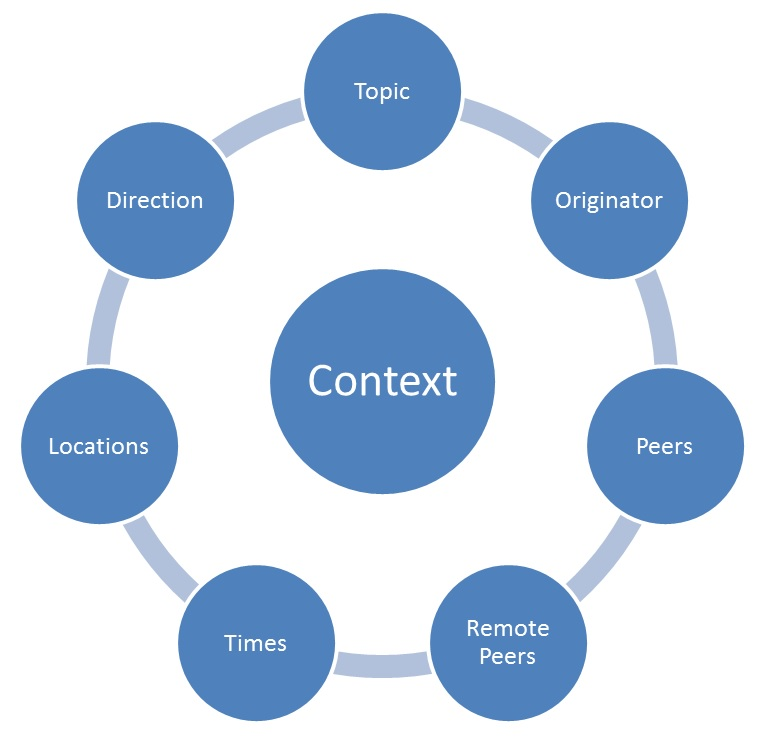
\includegraphics[width=\linewidth]{../Bilder/contextspace.jpg}
		\caption{Shark Context Space Modell}
		\label{fig:CSModel}
	\end{figure}
	
	Die einzelnen Elemente haben dabei folgende Bedeutung:
	\begin{itemize}
		\item \textbf{Topic:} Dies ist das Thema eines Kontextes. Es ist ist eine
		Beschreibung was der Kontext bedeutet.
		\item \textbf{Orginator:} Der Autor der des beschrieben Kontextes. Die
		kann entweder der Ersteller der sein oder Autor der beiliegen
		Informationen. Bei einem wissenschaftlichen Artikel wäre dies der Autor
		des Titels.
		\item \textbf{Peers:} Peers kann unterschiedlich interpretiert werden.
		Zum einen kann es der Ersteller des Kontextes sein, der sich vom Autor
		der beiliegenden Informationen unterschieden kann. Zum anderen kann es
		der Besitzer des eines Kontextes sein, wobei Besitzer hier je nach 
		beiliegendem Fall anders interpretiert werden kann. Im Allgemeinen
		kommt die Interpretation dieser auf den vorliegenden Fall an.
		\item \textbf{Remote Peers:} Dies sind die Peers an welche der Kontext
		gesendet werden soll.
		\item \textbf{Times:} Eine Zeitinformation die je nach vorliegendem Fall
		anders Interpretiert weiden kann. Diese Dimension biete die Möglichkeit
		ein Zeitintervall anzugeben.
		\item \textbf{Locations:} Gibt einen Ort an. Diese Information kann je
		nach vorliegendem Fall anders interpretiert werden.
		\item \textbf{Direction:} Die Richtung der Kommunikation des Kontextes.
		Es ist möglich nur Informationen über einen Kontext zu empfangen, sie nur
		zu senden, zu lesen und senden und keine der genannten Aktionen
		durchzuführen.
	\end{itemize} 	
	
	Zu beachte ist, dass wenn von einem Kontext gesprochen wird, dann handelt es
	sich hierbei um eine Beschreibung einer Menge von Kontextpunkten. Diese
	Punkte haben den gleichen Aufbau wie in \autoref{fig:CSModel} gezeigt. Der 
	wesentliche Unterschied ist, dass ein Kontext eine Vielzahl von Inhalten,
	ausgenommen der Direction, besitzen kann. Wehrendessen besitzt der
	Kontextpunkt nur je genau einen Inhalt. Beispielhaft beschriebt der
	Kontextpunkt nur das Thema Java, während der Kontext Java und C++ beinhaltet.
	Die Dimensionen selbst werde als Kontextkoordinaten bezeichnet. Der 
	Kontextpunkt vereint Koordinaten und Informationen. Der Kontext wiederum
	ist eine Möglichkeit eine menge an Kontextpunkten aus einer zugrundeliegenden
	Wissensbasis zu extrahieren.
	
	\subsubsection{Knowledge Base} 
	Die Knowledge Base, zu deutsch Wissensbasis, ist Eine Sammlung von Wissen.
	Wissen ist dabei eine Menge an Informationen, die anhand von
	Kontextkoordinaten beschrieben sind. Die Vereinigung von Kontextkoordinaten
	und Informationen bildeten einen Kontextpunkt.\\
	
	Die Wissensbasis bietet die Möglichkeit Peers und Themen zu speichern, sowie
	die Themen in einer Taxonom einzuordnen. Der für die zu entwickelnde
	Softwarekomponente wichtige Punkt ist aber die Möglichkeit genannte
	Kontextpunkt in ihr zu speichern und anhand eines Kontextes zu extrahieren.
	Die Wissensbasis selbst kann hierbei ähnlich einer Datenbank angesehen werden.
	Ziel ist es Teilbereiche, sprich eine bestimmte Menge an Daten dieser, mit
	anderen Wissensbasen zu synchronisieren. Zu diesem Zweck gebt es bereits eine
	Implementierung, SyncKB genannt, auf der aufgebaut wird. \\
	
	Zusätzlich zu den genannten Eigenschaften gibt es die Properties an der
	Wissensbasis zu speichern. Dies sind Name-Wert-Paare, wobei sowohl Name 
	als auch Wert eine Zeichenkette ist.
	
	\subsubsection{SyncKB} 
	
	Leider gibt es, abgesehen der Javadoc Dokumentation, keine genaue
	Beschreibung der Funktionsweise der SyncKB. Daher soll hier auf die
	generelle Funktionsweise dieser eingegangen werden. Weitere Informationen
	können den Quellcode selbst entnommen werden, der im Github vom SharkFW
	zu finden ist. \cite{SyncKB}
	
	\section{Konzeption}	
	
	\subsection{Ein erweiterter Kontext}
	
	Die Context Spache aus dem Kapitel \ref{sec:CS} ist für unsere Anforderungen
	nicht ausreichend.
	
	\newpage
	
	\section{Quellenverzeichnis}	
	\printbibliography[type=online,heading=subbibliography,title={Webseiten}]
	\printbibliography[type=manual,heading=subbibliography,title={Handbücher}]
	\newpage
	
	\section{Abbildungsverzeichnis}
	\makeatletter
		\@starttoc{lof}% Print List of Figures
	\makeatother

\end{document}